%Chapter 5

\renewcommand{\thechapter}{5}

%TODO: Add better title
\chapter{System Implementation}
\label{ch:system_implementation}

Given its grandiose title, it may seem that the engineering behind the development of a planetary scale data storage system would require thousands of man-hours of professional software engineers and a highly structured development process.
In fact, this is not necessarily the case for two reasons.
First, data systems benefit from an existing global network topology and commercial frameworks for deploying applications.
This means that both the foundation and motivation for creating large geo-replicated systems exists, as described in Chapter~\ref{ch:architecture}.
Second, like the internet, complex global systems emerge through the composition of many simpler components following straight forward rules~\cite{internet}.
Instead of architecting a monolithic system, the design process is decomposed to reasoning about the behavior of single processes.

Fundamentally, each process in our system is an independent actor~\cite{actors,scala_actors,orleans} with storage, memory, and compute resources.
The primary purpose of an actor is to receive and respond to messages (events) from other actors by modifying the actor's internal state, creating new actors, or sending messages to other actors~\cite{hewitt_actors}.
The behavior of an actor depends solely on the order of messages received, making them an ideal model for programming consistency protocols.
A system is therefore composed of actors, and reasoning about the global behavior of the system requires only a description of the interactions that different actors in the system have.

The actor model allows us to decouple consistency behavior from application behavior.
Consistency behavior is defined in the messaging between actors, for example actors participating in hierarchical consensus provide consistency by voting for a leader and correctly committing commands from the leader based on majority votes.
Application behavior is defined by the internal state of the actor, for example the maintenance of a versioned key-value store.
We use this decoupling to construct three principle applications from our consistency-centric model: a key-value database, a ledger, and a file system, all distributed geographically.

In this chapter we will describe the details of our implementation.
First, we will describe the base requirements for all replicas, along with our assumptions concerning communication, security, processing and data storage.
We will also outline the details of our implementation of the consistency protocols described in previous chapters.
Both HC and federated consistency are based on object stores that can be sharded and managed independently, therefore we will principally describe operations in terms of a key/value store.
Finally we will describe the details of the applications we built on top of our consistency protocols and the base object store.

\section{Replicas}
\label{ch05_replicas}

The primary actor in our system is the \emph{replica}.
Replicas are independent processes that maintains a portion of the objects stored as well as a \emph{view} of the state of the entire system.
Each replica implements a shared-nothing architecture~\cite{shared_nothing} such that each replica has its own memory and disk space.
For practical purposes of fault tolerance, we generally assume that there is a one-to-one relationship between a replica and a disk so that a disk failure means only a single replica failure.
Replicas must be able to communicate with one another and may also \emph{serve} requests from clients.
By default we assume that all replicas in the system are addressable and that both clients and peers can send messages to all replicas in the network, barring failures.

A system is composed of multiple communicating replicas and is defined by the behavior the replicas.
For example, a totally replicated system is one where each replica stores a complete copy of all objects as in the primary-backup approach~\cite{primary_backup}, whereas a partially replicated system ensures durability such that multiple replicas store the same object but not all replicas store all objects as in the Google File System (GFS)~\cite{gfs}.
At the scale of a multi-region, globally deployed system, we assume that total replication is impractical and primarily consider the partial replication case.
However, we also assume that replicas maintain a view of the entire system, that is meta-data about the location and provenance of all objects, so as to direct client requests to the appropriate replica to serve requests.

We assume that replicas reside on trusted hosts with reliable communication and that failures are non-byzantine~\cite{byzantine-generals,byzantine_fault_tolerance}.
However, we do expect security to be a default component of a real-world implementation, particularly as many communication links travel across the internet.
Communication should be secured and authenticated with transport layer security (TLS)~\cite{tlsv1,tlsv2}.
TLS requires that each replica maintains a certificate and public key encryption to secure communications~\cite{rsa} and if each replica has its own certificate, then TLS can also be used to authenticate valid peers based on a central authority's shared certificate~\cite{tls_authentication}.
We also assume that data stored on disk should be encrypted.
We prefer per-replica encryption to ensure that data is loaded and stored from an in-memory cache as quickly as possible though we recognize that some applications require per-user encryption; it is beyond the scope of our system to provide it.

\begin{figure}
    \begin{center}
        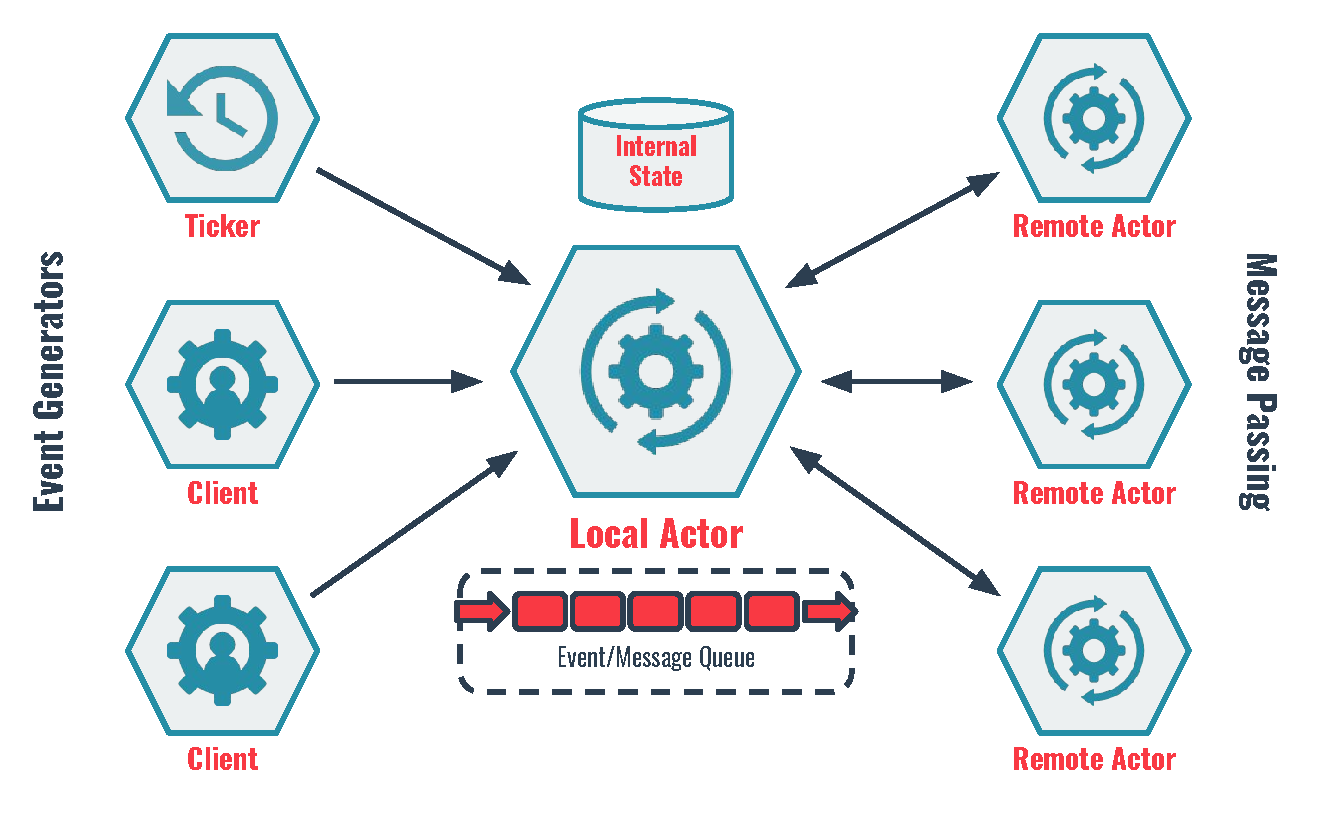
\includegraphics[width=5in]{figures/ch05_actor_model.pdf}
    \end{center}
    \renewcommand{\baselinestretch}{1}
    \small\normalsize

    \begin{quote}
        \caption[Replica Actor Model]{Each replica is an actor that maintains an internal state that is modified by processing messages from other actors. Implemented in the Go programming language, each event is serialized by a single message channel ensuring that the state is modified correctly.}
        \label{fig:ch05_actor_model}
    \end{quote}
\end{figure}
\renewcommand{\baselinestretch}{2}
\small\normalsize

All replicas are implemented in Go~\cite{golang}, a systems programming language that provides concurrency through communication channels~\cite{csp}.
Each replica implements a primary event loop as a single channel to ensure that all events and messages are serialized in a single order as shown in Figure~\ref{fig:ch05_actor_model}.
This prevents the need to use multiple expensive mutexes to synchronize the behavior of multiple threads and allows us to more easily reason about the operation of the system.
Communications are implemented using gRPC~\cite{grpc}, an HTTP communication protocol that serializes messages in the protocol buffers format~\cite{protocol_buffers} which allows clients to be implemented in multiple programming languages.
The gRPC server accepts new requests each in their own thread.
Clients are handled using unary RPC requests, but to improve communication performance between replicas we use bilateral streaming.
Each message is pushed through the primary event channel, then responded to using a callback channel.
Other threads include timers and monitoring threads that are also synchronized through the main event channel.

We've principally implemented two types of replicas with two different consistency protocols.
Alia~\cite{alia} replicas implement hierarchical consensus based on our implementation of the Raft protocol~\cite{alia_raft}.
Honu~\cite{honu} replicas implement eventual consistency using bilateral anti-entropy synchronization.
Both Alia and Honu implement an object store such that objects are described by unique keys, and each update to the object creates a new version.
The key/value nature of our implementation allows the namespace and object data to be sharded and partially replicated across all replicas, therefore the key/value database described in \S~\ref{ch05_key_value_db} is the base application for all of our applications.

Replicas primarily cache their object stores in memory to improve performance.
If a replica fails it can be brought up to date by a peer replica through either consistency protocol.
Durable storage is written to asynchronously, to minimize the amount of recovery time required for a replica.
Both Alia and Honu can use multiple backend stores, writing pages and logs to disk, or using embedded key/value stores such as LevelDB~\cite{leveldb}, BadgerDB~\cite{badgerdb}, or PebblesDB~\cite{pebblesdb}.
These databases use the ext4 file system, though in the future we hope to investigate the use of a tree-based file system to more directly optimize disk usage~\cite{btrfs}.

\subsection{Alia}
\label{ch05_alia}

Hierarchical Consensus with modified Raft as the underlying consensus
protocol exports a linearizable order of accesses to the distributed key-value
store.
Alia and the HC library are implemented in Golang use gRPC~\cite{grpc} for
communication.
The system is implemented in \todo{7,924 lines of code}, not including standard
libraries or support packages.

A replica implements multiple instantiations of the Raft protocol, which we have modified in several ways.
Every replica must run one instantiation of the \textit{root consensus protocol}.
Replicas may also run one or more instantiations of the \textit{commit consensus protocol} if they are assigned to a subquorum.
Repartition decisions move the system between epochs with a new configuration and tagspace, and can only be initiated by messages from peers or monitoring processes.
A successful repartition results in a new epoch, tagspace, and subquorum topology committed to the root log.
\texttt{Repartition} messages also serve to notify the network about events that do not require an epoch change, such as the election of a new subquorum leader or bringing a failed node back online.

\begin{figure}
    \begin{center}
        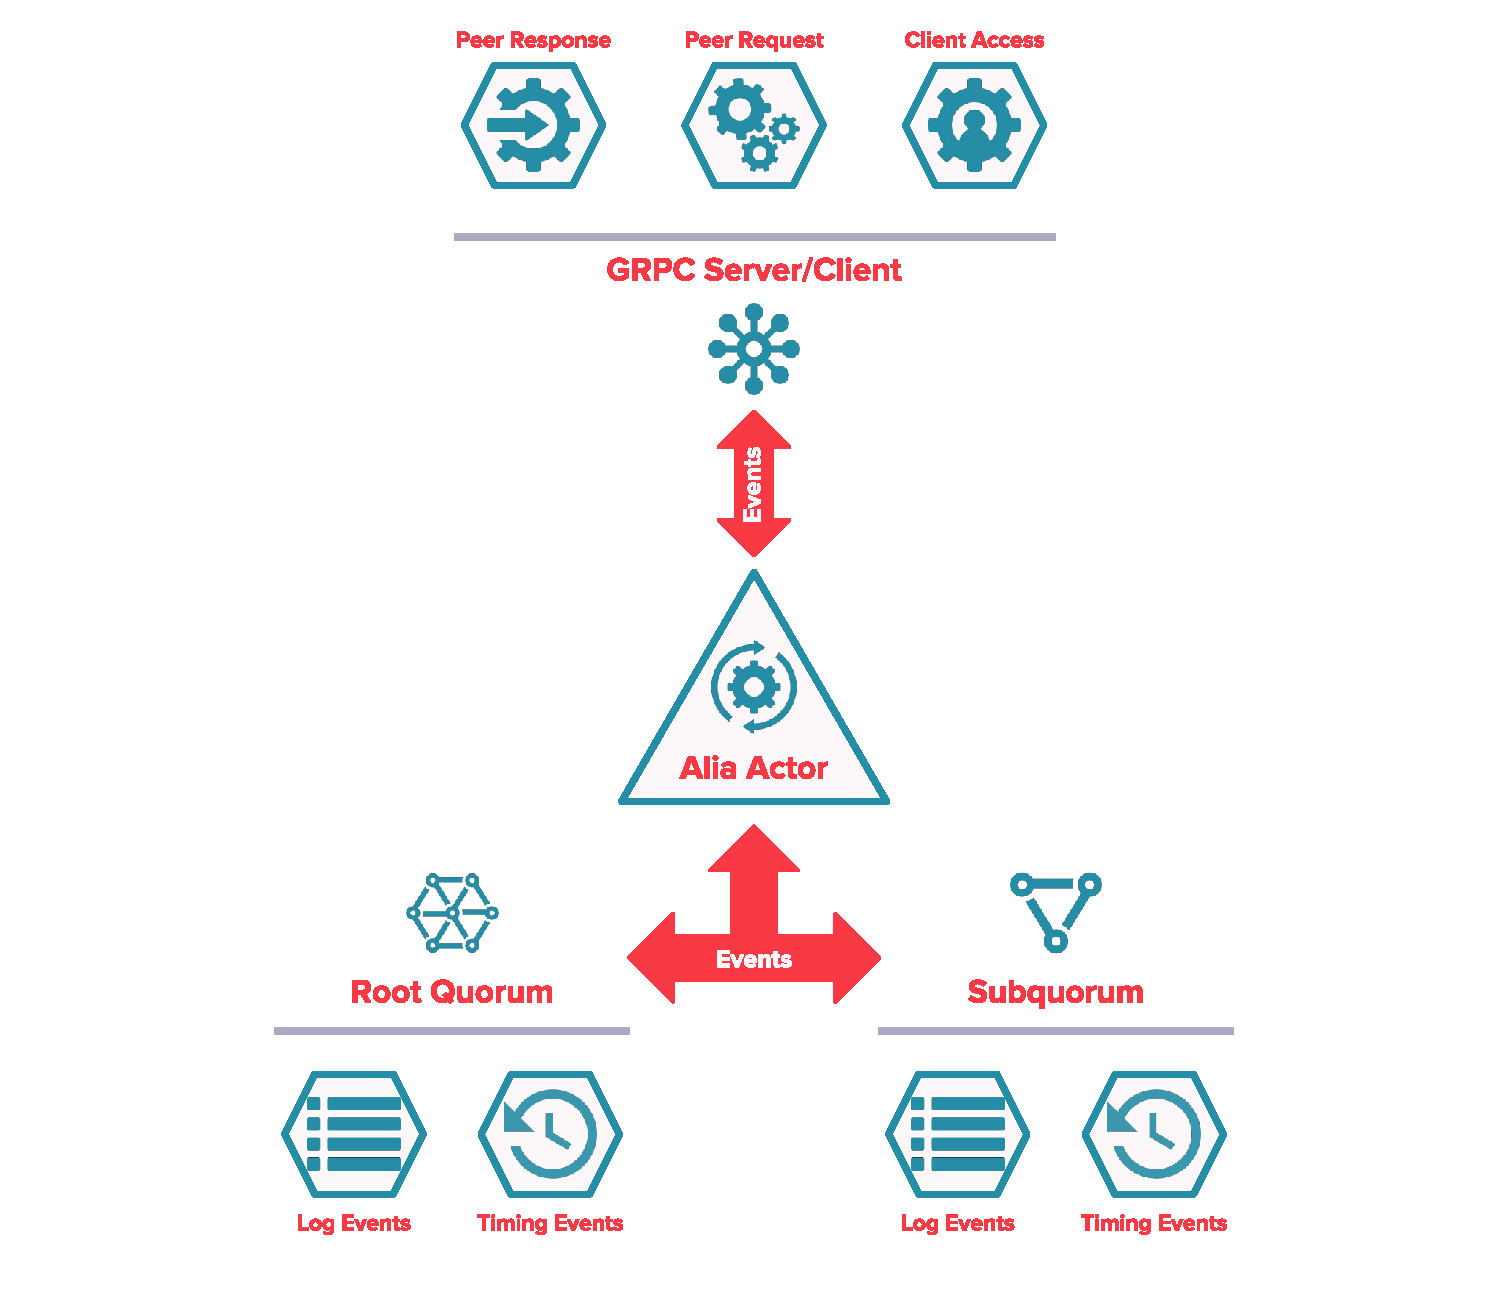
\includegraphics[width=5in]{figures/ch05_hc_actor_model.pdf}
    \end{center}
    \renewcommand{\baselinestretch}{1}
    \small\normalsize

    \begin{quote}
        \caption[Alia Actor Model]{The Alia actor model model is composed of at least three primary actors: the root quorum actor, a subquorum actor, and the main actor that dispatches messages to each subquorum. Other minor actors such as client requests threads and timing events dispatch their messages directly to their associated actors.}
        \label{fig:ch05_hc_actor_model}
    \end{quote}
\end{figure}
\renewcommand{\baselinestretch}{2}
\small\normalsize

Each replica implements an event loop that responds to timing events,
client requests, and messages from peers.
Events may cause the replica to change state, modify a command log, broadcast
messages to peers, modify the key-value store, or respond to a client.
% Events must be handled one at a time in the order they arrive at the replica
% to ensure correct behavior.
Event
handlers need to aggressively lock shared state for correctness because Golang and
gRPC make extensive use of multi-threading.
% This conflicts with the need to avoid complete serialization by exploiting concurrency.
The balance between correctness and concurrency-driven performance leads to
increasing complexity and tighter coupling between components, one that
foreshadows extra-process consistency concerns that have been noted in other
work~\cite{paxos_live,raft,raft_students_guide}.

The computing and network environment of a distributed system
plays a large role in determining not just the performance of the system, but
also its behavior.
A simple example is the election timeout parameter of the Raft consensus
protocol, which must be much greater than the average time to
broadcast and receive responses, and much less than the mean time
between failures~\cite{raft,etcd_raft,oliveira_evaluating_2016}.
If this requirement is not met,
leader may be displaced before heartbeat messages arrive, or the system will be
unable to recover when a leader fails.
As a result, the relationship between timeouts is critically dependent on the mean
latency ($\lambda_{\mu}$) of the network.
Howard~\cite{raft_refloated} proposes  $T = \lambda_{\mu} +
2\lambda_{\sigma}$ to determine timeouts based on the distribution of observed
latencies, sets the heartbeat as $\frac {T} {2}$, and the election timeout as
the interval $U(T,2T)$.
We parameterize our timeouts (Table~\ref{tab:ticks}) on
latency measurements made before we ran our experiments.
Monitoring and adapting to network conditions is part of ongoing work.


\renewcommand{\baselinestretch}{1}
\small\normalsize
 \begin{table}[ht]
\caption[Parameterized Timeouts of Raft Implementation]{Parameterized timeouts in our implementation. The \emph{obligation} timeout
  stops a partitioned subquorum after an extended time without contact to the
  rest of the system. $T=10 msec$ for our experiments on Amazon EC2.}
\begin{center}
\begin{tabular}{l|l|l}
\hline
Name & Time & Actions \\
\hline \hline
sub heartbeat& 1T & sub leader heartbeat\\
sub leader & 2-4T & new sub election\\ \hline
root heartbeat & 10T & root leader heartbeat \\
root election & 20-40T & new root election \\ \hline
obligation & 50T & root quorum may re- \\
 &  & allocate the tag \\
\hline
\end{tabular}
\end{center}
\label{tab:ticks}
\end{table}
 \renewcommand{\baselinestretch}{2}
\small\normalsize

\textbf{Changes to base Raft:} In addition to major changes, such allowing
replicas to be part of multiple quorums simultaneously, we also made many
smaller changes that had pervasive effects.
One change was including the \textit{epoch} number alongside the term in all
log entries.
The epoch is evaluated for invariants such as whether or not a replica can
append an entry or if a log is as up to date as a remote log.

Vote delegation requires changes to vote counting.
Since our root quorum membership actually consists of the entire system, all replicas
are messaged during root events.
All replicas reply, though most with a ``zero votes'' acknowledgment.
The root uses observed vote distributions to inform the ordering of future
consensus messages (sending requests first to replicas with votes to cast),
and uses timeouts to move non-responsive replicas into ``hot spares'' status.

We allow \texttt{AppendEntries} requests in subquorums to aggregate multiple client
requests into a single consensus round.
Such requests are collected while an outstanding commit round is ongoing, then
sent together when that round completes.
The root quorum also aggregates all requests within a minimum interval into a single
new epoch-change/reconfiguration operation to minimize disruption.

Commits are observed by the leader once a majority of replicas respond
positively.
Other replicas learn about the commit only on the next message or heartbeat.
Root epoch changes and heartbeats are designed to be rare, meaning that epoch
change commits are not seen promptly.
We modified the root protocol to inform subquorums of the change by sending an
additional heartbeat immediately after it observes a commit.

Replicas may be part of both a subquorum and the root quorum, and across epoch boundaries
may be part of multiple subquorums.
In principle, a high performance replica may participate in any number of
subquorums.
We therefore allow replicas to accommodate multiple distinct logs with
different access characteristics.

Peers that are either slow or with unsteady connectivity are occasionally left
behind at subquorum leader or epoch changes.
Root heartbeats containing the current system configuration are broadcast to
all replicas and serve to bring them up to date.

Finally, consensus protocols often synchronously write state to disk before
responding to remote requests.
This allows replicas that merely crash to reboot and rejoin the ongoing
computation after recovering state from disk.
Otherwise, these replicas need to go through heavyweight leave-and-rejoin
handshakes.
Our system avoids these synchronous writes by allowing epochs to re-join a
subquorum at the next epoch change without any saved state, avoiding these
handshakes altogether.

\subsection{Honu}
\label{ch05_honu}

\section{Applications}
\label{ch05_applications}

\begin{landscape}
\begin{figure}
    \begin{center}
        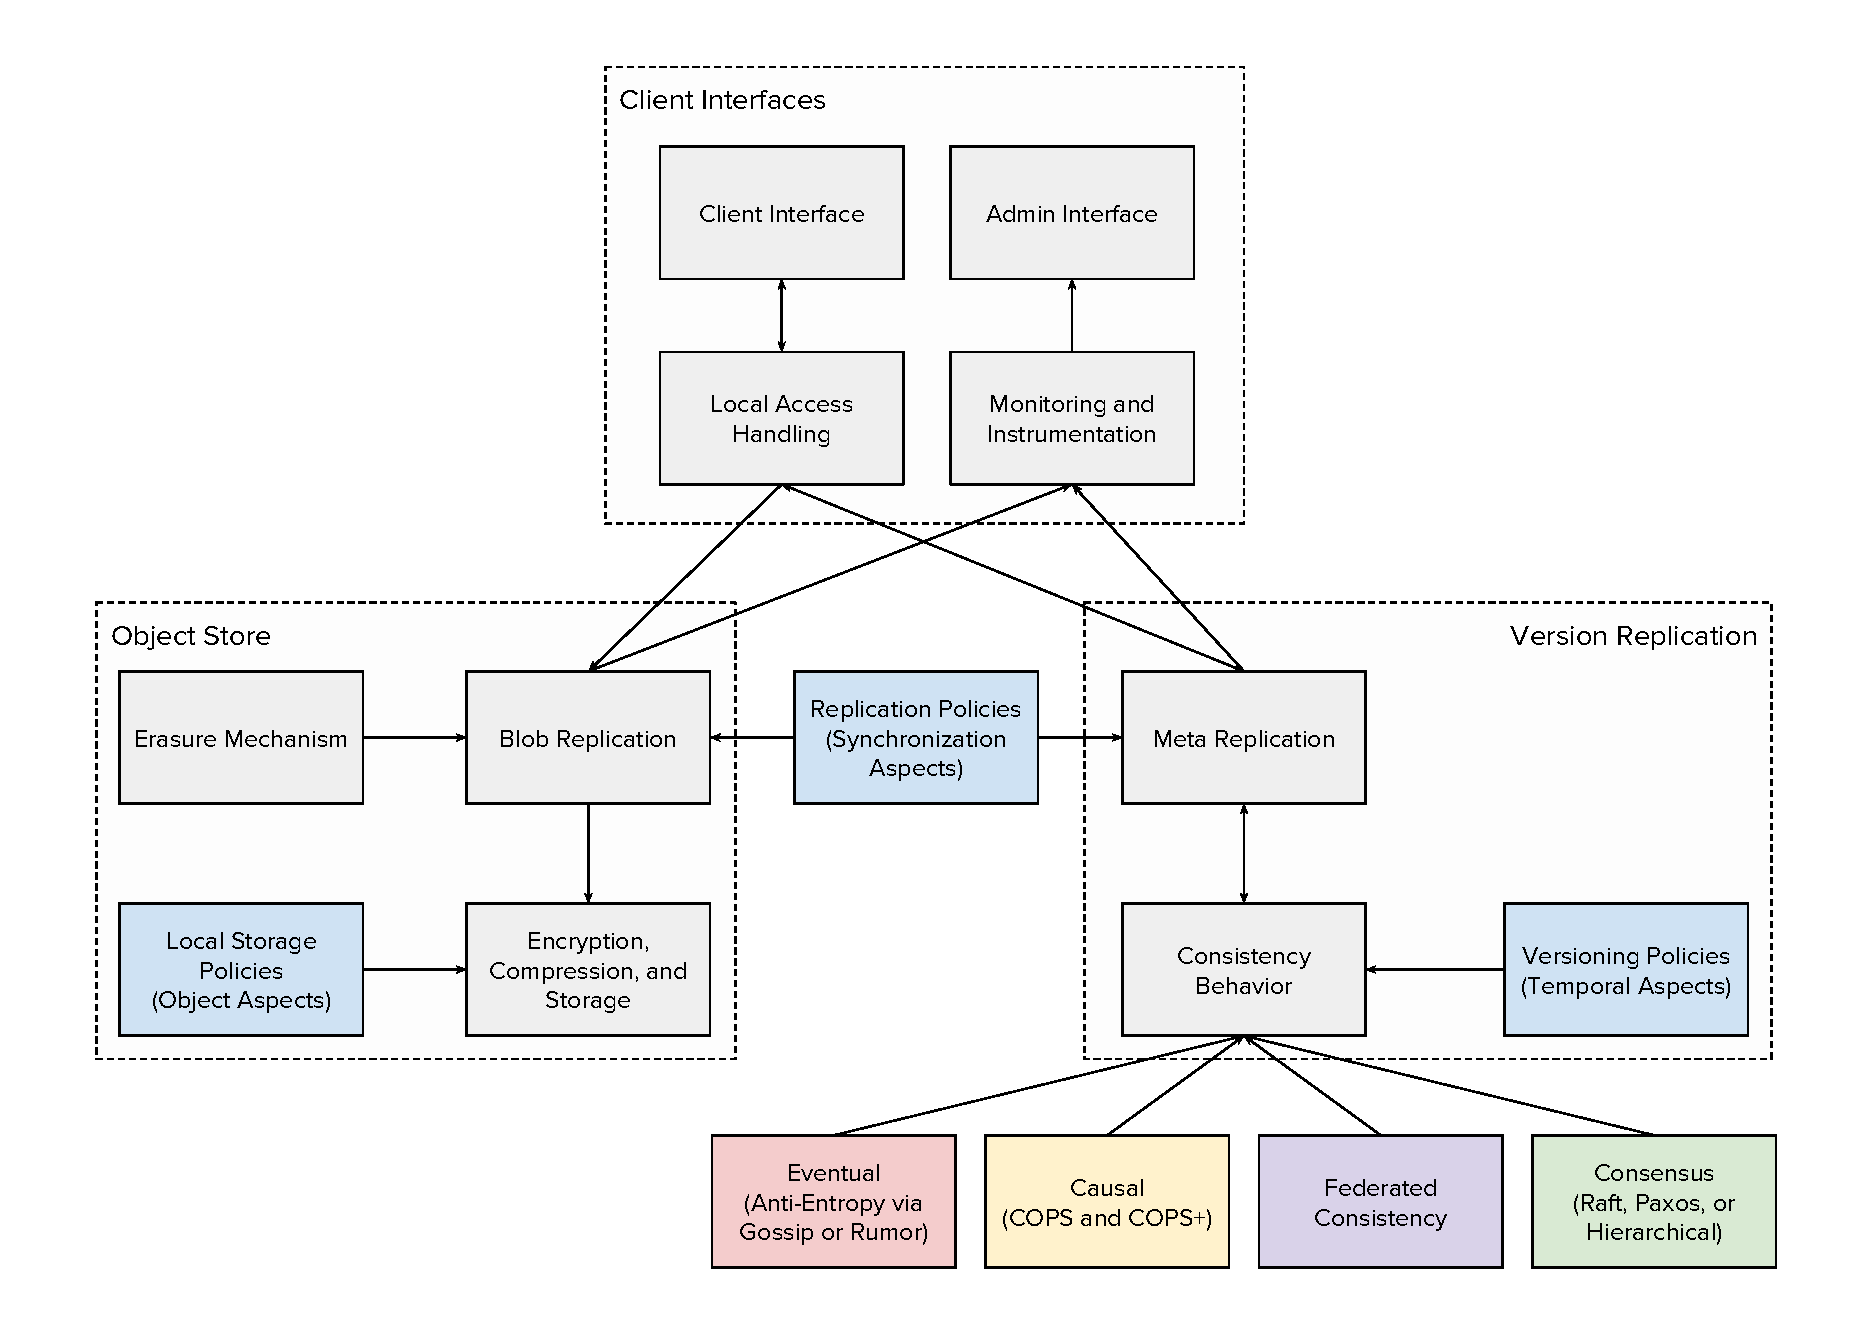
\includegraphics[width=7.2in]{figures/ch05_fluidfs_components.pdf}
    \end{center}
    \renewcommand{\baselinestretch}{1}
    \small\normalsize

    \begin{quote}
        \caption[Application Component Model]{This architecture provides a general component model for consistency-centric applications. Object blobs and version metadata are replicated separately to allow partial replication of data but a full view of the current state of the system. Only version replication requires consistency semantics, therefore our federated and hierarchical consensus models only deal with metadata commands.}
        \label{fig:ch05_fluidfs_components}
    \end{quote}
\end{figure}
\renewcommand{\baselinestretch}{2}
\small\normalsize
\end{landscape}

\subsection{Key-Value Database}
\label{ch05_key_value_db}

\subsection{File System}
\label{ch05_file_system}

In the context of a wide-area file system, those operations could be individual
\texttt{write()} systems calls, though this would be inefficient.
Most wide-area file systems aggregate individual accesses through
\textit{Close-To-Open} (CTO) consistency, where file reads and writes are
``whole file'' \cite{afs,coda,lbfs}.
A file read (``open'') is guaranteed to see data written by the latest write
(``close'').
This approach satisfies two of the major tenets of session consistency:
\texttt{read-your-writes} and
\texttt{monotonic-writes}, but not
\texttt{writes-follow-reads}~\cite{bermbach_consistency_2013,anti_entropy,eventual_consistency}.

Our file system, like many modern file systems,
decouples
meta-data~\emph{recipes}~\cite{casper,gfs,hadoop_hdfs,pvfs,globalfs}
from file
data storage.
Meta-data includes an ordered list of \emph{blobs}, which are opaque binary chunks.
When a file is closed after editing, the data associated with the file is \emph{chunked} into a
series of variable-length blobs~\cite{lbfs}, identified by a hashing function applied to
the data~\cite{rabin_karp,rabin_fingerprint}.
Since blobs are effectively immutable~\cite{immutability_changes_everything}, or tamper-evident, (blobs are named by hashes of
their contents), we assert that consistent meta-data replication can be decoupled from blob
replication.
Accesses to file system meta-data becomes the operations or entries in replicated logs.
Meta-data is therefore replicated through the system, allowing any file
system client to have a complete view of the file system namespace, even while
not caching any file data.

\begin{landscape}
\begin{figure}
    \begin{center}
        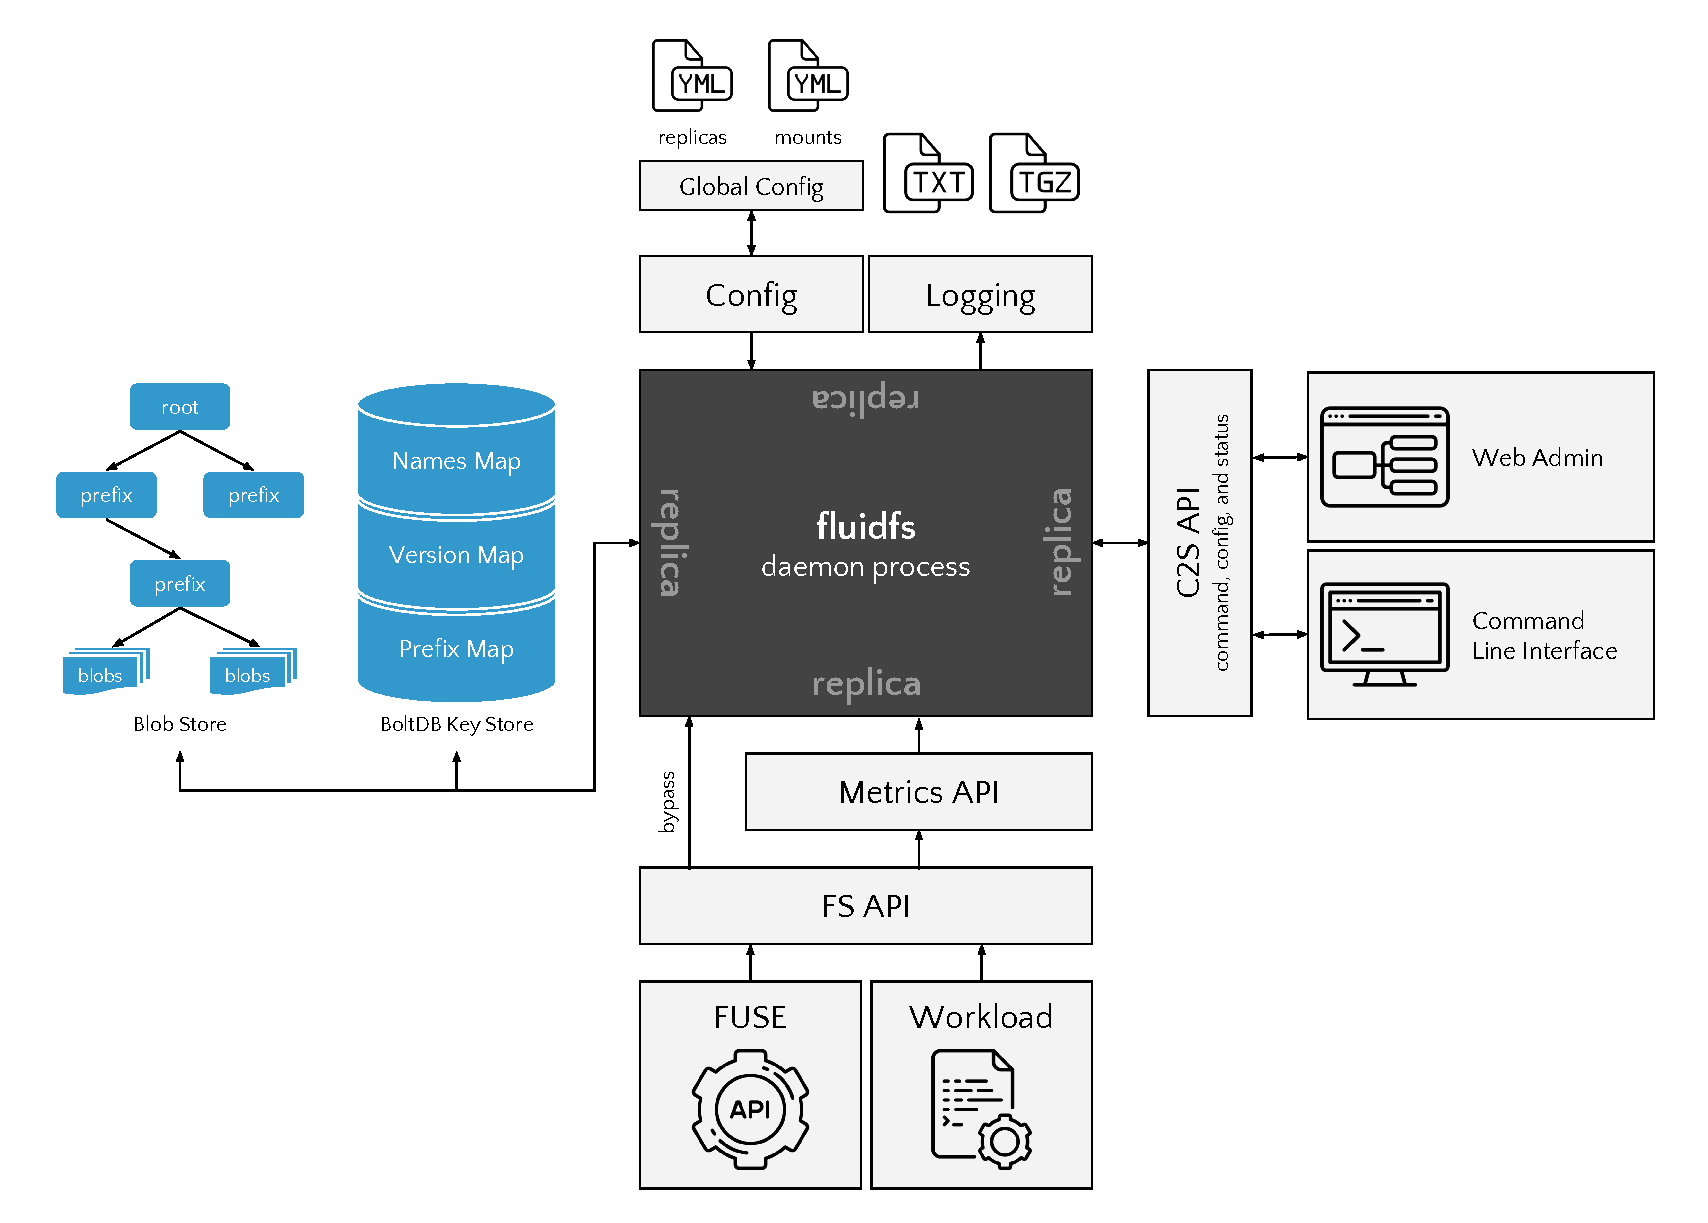
\includegraphics[width=7.2in]{figures/ch05_fluidfs_replica.pdf}
    \end{center}
    \renewcommand{\baselinestretch}{1}
    \small\normalsize

    \begin{quote}
        \caption[FluidFS Architecture]{FluidFS implements the application component model specifically for a file system. Users interact with a local replica that implements the FUSE API or more directly through a gRPC API. The FluidFS daemon process stores data in a blob store and meta data in an embedded key/value store. The process also provides configuration and logging as well as a web interface for command and control.}
        \label{fig:ch05_fluidfs_replica}
    \end{quote}
\end{figure}
\renewcommand{\baselinestretch}{2}
\small\normalsize
\end{landscape}

\subsection{Distributed Ledger}
\label{ch05_distributed_ledger}

\section{Conclusion}
\label{ch05_conclusion}

We did not optimize our research for the minimum set of assumptions required to facilitate interoperability between heterogeneous replicas.
However, we hope that the assumptions we did make shed light on what is required to achieve the minimum set of assumptions.

Further research is required to ...
